%Emma Callery's Senior Seminar Paper

\documentclass{sig-alternate}
\usepackage{color}
\usepackage{listings}
\usepackage{url}
\usepackage{natbib}
\usepackage{graphicx}

\begin{document}
\conferenceinfo{UMM CSci Senior Seminar Conference, December 2014}{Morris, MN}
\title{Static and Dynamic Types in Software Development}
\numberofauthors{1}
\author{
\alignauthor
Emma G. Callery\\
	\affaddr{Division of Science and Mathematics}\\
	\affaddr{University of Minnesota, Morris}\\
	\affaddr{Morris, Minnesota, USA 56267}\\
	\email{calle052@morris.umn.edu}
}

\maketitle

\begin{abstract}
The debate between statically and dynamically typed languages has been going on since programming languages were first introduced. Arguments for the different types have gone back and forth on everything; from the benefits of both type systems to what makes programmers hate one of the type system or the other. Unfortunately most arguments made for and against both type systems tend to come from personal opinions or personal experience. 
This paper takes a look at several studies that have tried to look at this debate empirically to determine if either type system has an greater benefit to programmers using it. The first study looked at how programmers prefer to incorporate types in their programs when they have the chose of including them. Several other studies have compared the time required to write out similar code in both a static and a dynamic language. 
The results show that the language which provides the greater benefit depends not only on the kind of programming task being completed but also on the programmer writing the code. While there are times where a static type system is faster to write code in, there are other times dynamic typed systems are quicker to write and even times where it is hard to determine if there is any difference at all. This ultimately suggests that there is no `superior' type system. 
\end{abstract}

\keywords{Static Types, Dynamic Types, Programming Languages, Java, Groovy.}

\section{Introduction}\label{intro}
Type systems (see \citep{Pierce2002}) have played an important role in programming languages since the first languages were developed. Type systems affect programmers in every level, from education to research to industry. While a great number of programming languages used in education are statically typed (e.g.,Java). A fair number of industry programs prefer use dynamically typed systems (e.g.,Groovy), especially for things like web development. This leads to the proposed question of "whether one system or another, either static or dynamic, has a larger benefit for the humans that use them"\cite{Mayer2012} then the draw backs that are argued by the other side. 

This question has lead to a large debate of the benefits and draw-backs of each of the type systems, with people arguing strongly for and against both. For example, there are some programmers that believe strongly that the structural benefits provided by static types out weighs the 'tediousness' or 'rigidity' that programmers that prefer dynamic types claim static types systems inherently have.   
Several recent studies have been conducted to try to determine if any of the arguments given by both sides have any real empirical support. 

This paper starts by defining what static and dynamic typed languages are in section \ref{types}, including commonly argued benefits for both. Section \ref{programmers} looks at a study that analyzed past projects to find patterns in how programmers use types. Two more studies have tried to look for empirical evidence to support the claim the static type systems have better trade-offs, their studies and results are in sections \ref{benifits} and \ref{influence}. We try to conclude an answer to the proposed questions in section \ref{results}.

\section{Background Information}\label{types}
This section defines static and dynamic types, as used in this paper, along with the common arguments for both type systems. %In addition the programming language Groovy is defined.

\subsection{Static Types}\label{static}
A language is said to be statically typed if the type of every variable is known by the compiler at compile-time. For the type to be known at compile-time the programmer has to have included the information required for the compiler to determine the type of the variable, which is done through several options, usually declaration. Static languages compilers enforce these types by only allowing values of the variable's type to be assigned to the variable. see Figure 1. This means that when the compiler goes through the code it not only checks other errors, but also checks for syntactic errors.
 
\subsubsection{Arguments For Static Types}\label{arguments}
%\begin{itemize}
%\item Most error checking is done at compiled-time, therefore catching errors more quickly.
%\item Types help to communicate to the programmer and the programmer reason about the program.
%\item Requiring type names act as a form of documentation or improves the quality of the documentation.
%\item Improve the programs structure.
%\end{itemize}
Type checking is one arguable benefits of static types. Since this checking is done at compile-time, the errors are more likely to be caught quickly and without having to run the whole program as frequently. A second common argument is that types improve the structure of a program. Better structure is believed to help the programmer reason about the program. The last significant argument for static types is that the types provide a form of documentation that can communicate to programmer. When the documentation from the types is added to the documentation written by the programmer it will, in theory, return a documentation of greater quality.

\begin{figure}
\centering
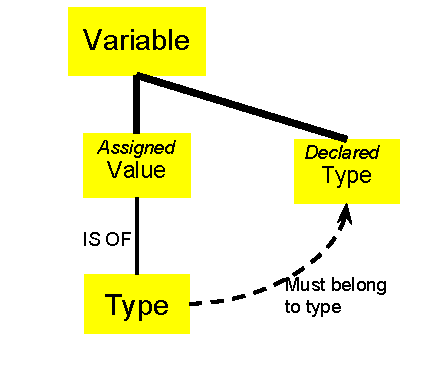
\psfig{file=Static_Type_Diagram.pdf,width =2in}
\caption{Diagram of Static Types and Type Checking \cite{Ferg2012}}
\end{figure}

\subsection{Dynamic Types} \label{dynamic}
``A language is dynamically typed if the type of a variable is interpreted at run-time''\cite{NomeN2009}. This is because types in dynamic languages are only associated with values\cite{Pierce2002}, as shown in Figure 2. This does not mean that a type can not be associated with a variable, only that the language would not require the type be declared. This \emph{option} leads to what is called \emph{optional typing} where the programmer is primarily  responsible for the types incorporated in the program, as explained in section \ref{programmers}. 

\subsubsection{Arguments for Dynamic Types}
%\begin{itemize}
%\item More flexible, variables can be passed between functions more easily.
%\item Without the need to declare every variable will make the program shorter, and therefore faster to write and read.
%\item Programs without specific type requirements can be easily reused, with out having to write a whole new function to do the same thing to a different type
%\item Not needing to declare variables, along with other 'administrative' commands, just to keep the compiler running allows for focusing to the conceptual concepts of the program.
%\end{itemize}
Not being required to type every variable is argued to make dynamically typed programs shorter and therefor faster to write and read. Dynamic types are also argued to allow greater flexibility to the programmer. There are several reason for this including easier passing of variables between different parts of a program. No specific type requirements allow for easier reuseability of part of programs. Declaring variables is considered 'administrative' and would allow for the programmer to focus on the more conceptual aspects of the program.

\begin{figure}
\centering
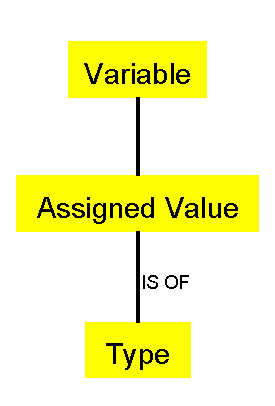
\psfig{file=Dynamic_Type_Diagram.pdf,width =1in}
\caption{Diagram of Dynamic Types \cite{Ferg2012}}
\end{figure}

\section{Programmer Preferences} \label{programmers}
This section will look at a study which attempted to determine where programmers use types and what types they used. The language used is the optional-type language \emph{Groovy}. Groovy is actually dynamically typed language created for the Java Virtual Machine. Because of this programmers using Groovy can access the static types within Java while also having the additional features found in other dynamic programming languages. This results in Groovy becoming an optional-type language where a programmer can include a static type declaration or use the dynamic type default, \emph{def}.

\subsection{Study on Optional Typing}
Carlos Souza and Eduardo Figueiredo studied programmer preferences in their paper \emph{How do Programmers Use Optional Typing? An Empirical Study}. In this study Souza and Figueiredo looked at 6638 open source projects written in Groovy, all gathered from Github. For each project Souza and Figueiredo gathered the source code, the commit history for the project, and the metadata for both the source code and all programmers involved in the project.
The source code metadata included the kinds of type declaration, if the declaration was public,private or protected. The programmer metadata primarily included their past language experience.

Looking over all of the projects Souza and Figueiredo tried to answer several questions about the use of types in the different projects. The questions were: 
\begin{enumerate}
\item \label{interface} ``Do programmers use types more often in the interface of their modules?''
\item \label{tests} ``Do programmers use types less often in test classes and scripts?''
\item \label{experience} ``Does the experience of programmers with other languages influence their choice of types in their code?''
\item \label{sizeageactivity} ``Does the size, age or level of activity of a project have any influence on the usage of types?''
\item \label{changed} ``In frequently changed code, do developers prefer typed or untyped declaration?'' 
\end{enumerate}
After collecting data from all the projects Souza and Figueiredo sorted the data by different measures. The measures were the kind of type declaration, the visibility of the declaration, the usage of the different types and where. Also used to sort the collected data was the size of the project in lines of code, the age of the program along with the number and frequency of commits. It was from this data and different comparisons that Souza and Figueiredo attempted to answer their hypotheses.

\subsection{Results for Optional Typing Study}
Question \ref{interface} was found to be true; variables and fields that are public, such as constructor and method parameters and returns, are frequently typed, see Figure \ref{Usage}. In addition the visibility of the declaration is also important. Souza and Fiqueiredo found that protected declarations are almost always typed and while public declarations are not as frequently typed as protected, they are typed more than private declarations, see Figure \ref{Visibility}. Though the reason for why module interface definitions are most often typed is still unresolved; Souza and Fiqueiredo suggest that the implicit documentation the types provide are the main incentive as programmers may consider documentation in these area important.

\begin{figure}
\centering
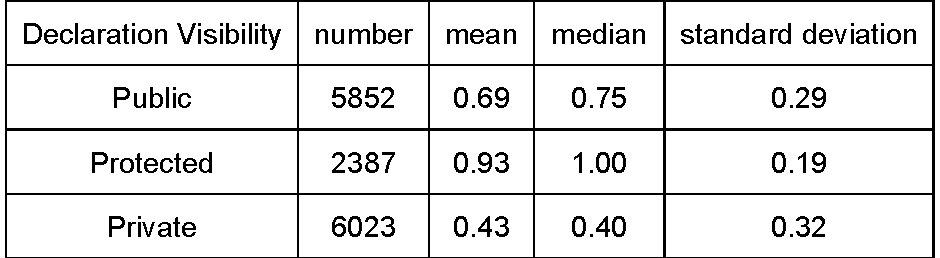
\psfig{file=Declaration_Visibility.pdf,width =2.8in}
\caption{Visibility of type declarations}
\label{Visibility}
\end{figure}

\begin{figure}
\centering
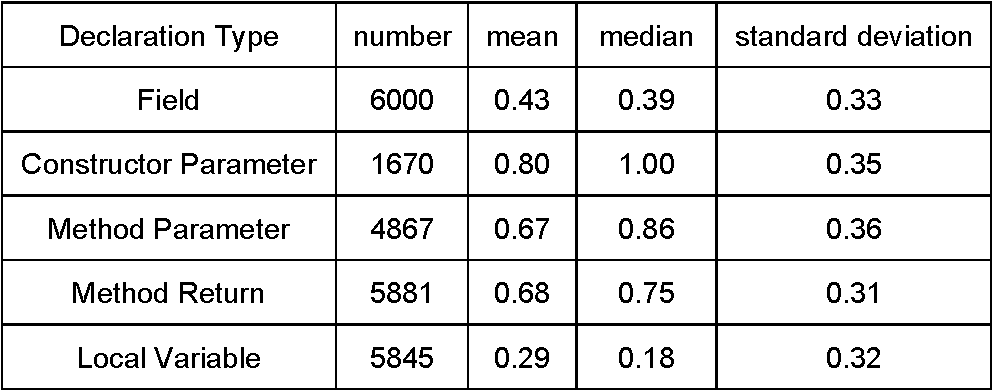
\psfig{file=Type_Declaration_Usage.pdf,width =2.8in}
\caption{Type declaration usage}
\label{Usage}
\end{figure}

%\resizebox{3.4in}{!}{
%\begin{table}[h]
%\begin{tabular}{|c|c|c|c|c|}
%\hline
%Declaration Tpe & Num. & Mean & Median & Std. Div. \\ \hline
%Field & 6000 & 0.43 & 0.39 & 0.33 \\ \hline
%Constructor Parameters & 1670 & 0.80 & 1.00 & 0.35 \\ \hline
%Method Parameters & 4867 & 0.67 & 0.86 & 0.36 \\ \hline
%Method Return & 5881 & 0.68 & 0.75 & 0.31 \\ \hline
%Local Variable & 5845 & 0.29 & 0.18 & 0.32 \\ \hline
%\end{tabular}
%\caption{Type declaration usage}
%\label{Usage}
%\end{table}
%}

On the other hand, question \ref{tests} was found to be false. Documentation is rarely needed for test classes and scripts as most are small and easy to understand already. Test classes tend to have one sole purpose, and are very rarely reused. While scripts can not be accessed by other modules so the type being passed is most likely already known. 

Unsurprisingly, question \ref{experience} was true. How a programmer uses types in an optional language greatly reflects how that programmer used types in other languages. Programmers coming from a statically typed language are more likely to add types than programmers coming from a dynamically typed language, see Figure \ref{Background}. It has been found that programmer become comfortable in whatever language they use most frequently.

\begin{figure}
\centering
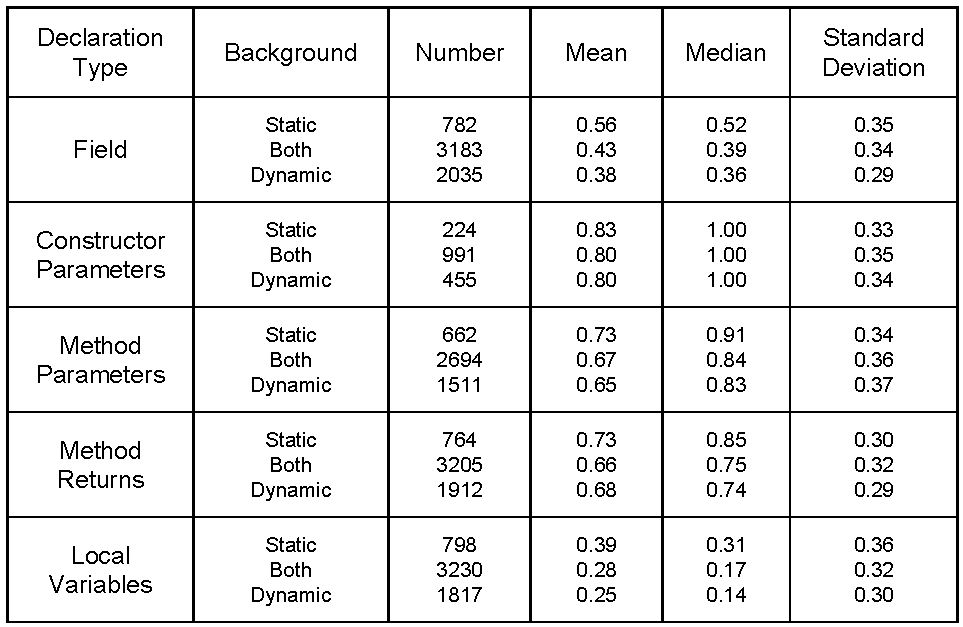
\psfig{file=Programmer_background_Usage.pdf,width =3.4in}
\caption{Type declaration usage by programmer background}
\label{Background}
\end{figure}

Souza and Figueiredo initially believed that as time goes on and the projects grow and \emph{mature}, the maintenance of projects becomes more difficult. This leads programmers to use more types as a means to make code more readable. A mature project was defined as ``a project that is 100 days old or more and has, at least, 2K LoC [Lines of Code] and 100 commits.''\cite{Souza2014}
The data gathered to try to answer question, shown in Figures \ref{Maturetype} and \ref{Matureview}, however, showed that this was not the case. Souza and Figueiredo thought that maybe the data they gathered could not ``actually correlate to the need for maintenance'' or if the data could work ``programmers might not have the opportunity or desire to make their code more maintainable'' \cite{Souza2014}.
\begin{figure}
\centering
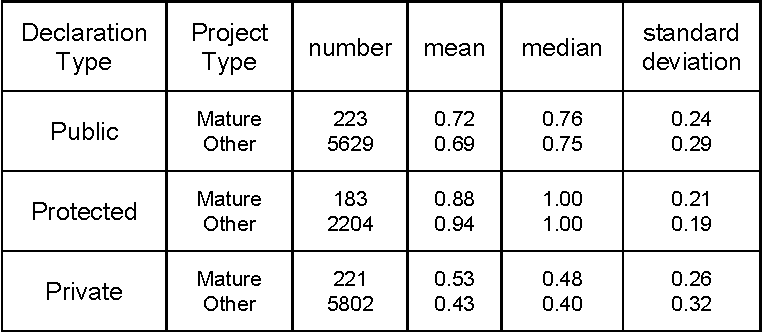
\psfig{file=Mature-Projects_View.pdf,width =2.8in}
\caption{Type declaration usage by project maturity}
\label{Maturetype}
\end{figure}
\begin{figure}
\centering
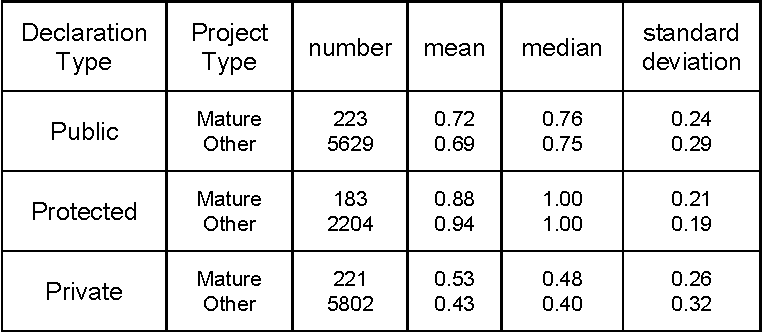
\psfig{file=Mature-Projects_View.pdf,width =2.8in}
\caption{Type visibility usage by project maturity}
\label{Matureview}
\end{figure}

Question \ref{changed} probably has the biggest debate attached to it. That being the argument that types, acting as a form of documentation, could make frequently changed code easier to change. Others argue that untyped code, being simpler, can be changed faster. It is this latter argument that Souza and Figueiredo found evidence for. They found that as changes in a file increase in frequency, 65\% of the mature projects showed a preference for the use of untyped declarations.

Overall this means that programmers are influenced by the type system that they are use to. Generally, programmers mostly type the definitions of a modules interface more frequently than anything else. Programmers also tend to omit types when they have to keep making changes to pieces of code. However this means that this debate of static vs dynamic types needs to be looked at more closely to determine if there is an actual benefit to one type system over the other. For this the two paper discussed in the following sections studied. 

\section{Influence of Static Types}\label{influence}
This section looks at a study conducted by Stefan Hanenberg, Clemens Mayer, Romain Robbes, Andreas Stefik, and Eric Taner in their paper \emph{An Empirical Study of the Influence of Static Type Systems on the Usability of Undocumented Software} \cite{Mayer2012}. This study looked into the argument that types act as a form of documentation, as a benefit of static type systems. The study argues that if there is no other form of documentation present and variables are not typed, it should take a programmer longer to complete a task than if the variables are typed. 

The researcher came up with two null hypotheses, the first stating that, 
\begin{quote}
Yhe development time for completing a programming task in an undocumented API is equivalent when using either a static type system of a dynamic type system.\cite{Mayer2012}
\end{quote} Because this hypothesis only accounts for the design of the API as a whole, null hypothesis two was included. Null hypothesis two states that,
\begin{quote}
There is no difference in respect to development time between static and dynamic type systems, despite the number and complexity of type declarations in an undocumented API. \cite{Mayer2012}
\end{quote} 
Both hypotheses were used so that if either hypothesis is rejected by the data, insight can be gained on the relative benefits and consequences of both type systems.

In the case of this study an undocumented API means that the interfaces used by the subjects had no documentation available to tell what exactly the interfaces did and which parameters needed to be passed to the methods within the API. It should be noted that the dynamic API used in this study was made by taking the static API and removing the type annotation; replacing them with the Groovy default, \emph{def}. This posses a potential problem with the study methodology in that this does not use any of the possible features of dynamically typed languages.

 
\subsection{Experiment}
The experiment designed for this study had 27 subjects that had  experience with the chosen static language, Java, but had no experience with the chosen dynamic language Groovy, which in this case was restricted to be a purely dynamic equivalent to Java. As all the subjects had experience with Java but no experience with Groovy, the authors simply introduced the subjects to Groovy as "a Java version where all declarations of variables, parameters, etc. only required the keyword \emph{def}." \cite{Mayer2012} 

While a learning effect was a potential issue to the validity of the experiment; this experiment design has already been applied to other studies successfully. In addition there are valid approaches for statistically analyzing the data fairly. So long as the learning effect is less than the effect caused by the language then the measures can still be used to determine the effect of the language.

Subjects were separated into two groups, as evenly as possible, and each group was asked to complete the same five programming tasks. The five tasks were completed in one language using one undocumented API before completing the five tasks in the second language with another API. Group one (called GroovyFirst) would complete the first set of assigned tasks using Groovy and then complete the tasks using Java. The other group (called JavaFirst) did the same tasks but did the tasks in Java first. 

The tasks were designed to vary in difficulty and the number of type declarations required for classes within each language.
\begin{description}
\item[Task 1]\hfill \\ 
This task was of easy difficulty and only asked to return an instance of a specific class. This required only one type to be identified for and taking only one line of code to write.
\item[Task 2]\hfill \\ 
This task was also considered easy. It required the initialization of an object found in the class from task1. The initialization required an initializer, which required  a secondary object. This means that the subjects had to identify three classes.
\item[Task 3]\hfill \\
This task was considered medium difficulty and required subjects to create a transformation of a object, from task 2, with a corresponding class. To do this a graph first had to be created from the task 2 object. An initialization of a different object had to be created, along with a node. The node and both objects where then passed to the transformation class. This means that the subject had to identify three classes. 
\item[Task 4]\hfill \\
This task was the only task to be considered difficult. The subjects were required to add a node to a graph through parameterizing an non-trivial initializer correctly. The parameters required were an instance of a sequence object, each object contained an identifier and a sequence of pairs. These pairs contain an identifier and another sequence object. Despite the subject only needing to identify three classes, the recursive definition of the objects lead to a suspicion that the code may be hard to understand, especially in the dynamic type system, with no defined types. 
\item[Task 5]\hfill \\
This task was considered easy, but required the highest number of classes that needed to be identified. The subjects were required to take the object from task 2 and create method that takes a command object(also created) and makes a 'menu' from the task 2 object. This 'menu' method also takes three additional classes to fully complete the command. In total six classes needed to be identified.
\end{description} 

It is interesting to note is that one subject was removed from the experiment because it was found that the subject had ``spent a very large amount of time in reading the complete source code while working on task 2 and then solved tasks 3 and 4 quickly'' \cite{Mayer2012}. After this had been confirmed to be the case and that it was the way the subject worked the subjects data was removed. This indicates that different programmers have different ways of processing and writing code, meaning that there is no one way of programming that could work for everyone. 

\subsection{Results}
It should be noted that, for several reasons, the programming tasks were designed with the assumption that ``for all tasks, except task 1, the static type system would show a measurable positive impact''\cite{Mayer2012}.

\subsubsection{Null Hypotheses results}
After analysis of the collected time data it was found that, concerning the first hypothesis, tasks 1, 4, and 5 showed a positive impact for the static type system, Java. Tasks 2 and 3, however, showed a positive impact for the dynamic type system, Groovy, as seen in the first line of Figure \ref{influenceResults}. This caused hypothesis one to be rejected.
\begin{figure}
\centering
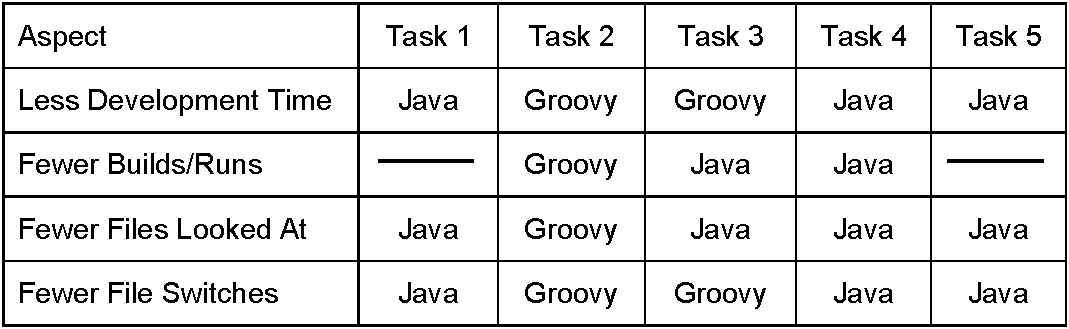
\psfig{file=Influence_Paper_Results.pdf,width =3.4in}
\caption{Collective results of all tasks showing leading language(either statically typed Java or dynamically typed Groovy)\cite{Mayer2012}}
\label{influenceResults}
\end{figure}

Hypothesis 2, however, cannot be rejected because the just the number of types and difficulty of the tasks ``cannot be a main effect of the difference between static and dynamic'' \cite{Mayer2012}. This is because for the 'easy' tasks(1,2,and 5) the dynamic type system was found to have a positive impact on only task 2, while tasks 1 and 5 showed a negative impact. This contradicted the assumption that the number of types needing to be identified is a main factor. Task 2 required more types to be identified than task 1 but less types than task 5. For tasks 3 and 4, which had the same number of type identifications required but different difficulties, contradictory results were also found.

\subsubsection{Exploratory Study and Results}
The contrary nature of the hypothesis 2 results lead to an investigation to find if other influences could have contributed to the results. One suggested influence was the measured number of builds and times tests were run during each task. These numbers were taken from the times the compiler ran and the times the 'start-button' was clicked. Tasks 1 and 5 registered no significant difference between Java and Groovy in number of builds and tests run. However tasks 3 and 4 showed the static type system, Java, had the fewer test runs. Task 2 was the only task where the dynamic type system, Groovy, had fewer test runs. The resutls as seen in second line of Figure \ref{influenceResults}.  

A second suggested factor was the number of files the subject was looking at, which may indicate the amount of the source code that a subject needed to read in order to complete the task. The authors assumed that this could have an effect because subjects using the dynamic system 'should' be more likely to look at unrelated source code. Evidence gathered seems to support this theory for all but one task, task 2. For tasks 1, 3, 4, and 5 fewer files were viewed when the subject was using Java. Task 2 showed that fewer files were viewed when the subjects used Groovy. See line three of Figure \ref{influenceResults}.

The final suggested factor was that the number of times the subject switched could indicate the amount of exploration the subject did while solving the task. Similarly to the previous suggestion, the effect was assumed to come from the 'required' need for user of a dynamically typed language to frequently change files to find or formulate answers. This was measured separately from the previous analysis. Oddly enough the results from this analysis directly correspond to the development time results, for each task. See line four of Figure \ref{influenceResults}. Tasks 1, 4, and 5 showed fewer file switches when the subjects used the static type system Java, while tasks 2 and 3 showed fewer files switched when subjects used the dynamic type system, Groovy. This result suggests that the number of switched files could be an indicator for the resulting development time. 

\section{Static Vs Dynamic Type Systems}\label{benifits}
This section discusses the study and results of Andreas Stuchlik and Stefan Hanenberg's study \emph{Static vs. Dynamic Type Systems: an Empirical Study About the Relationship between Type Casts and Development Time}\cite{Stuchlik2011}. The study was designed for the argument that, in simple programming tasks, the existence of type declarations leads to a reduction of development time. The reasoning behind this hypothesis is that including type declarations should lead to better development times, through types improving the program structure and the programmers' understanding.

\subsection{Experiment}
The study had 21 subjects, who were asked to complete two equivalent sets of programming tasks, with five programming tasks in each set. One set of tasks would be completed using Java and the other set using a restricted form of Groovy. The form of Groovy used in this study was restricted to a state of being the dynamic equivalent of Java, similar to the study above. Also like the study above, the subjects were split into two groups,as evenly as possible; one group started by completing one set of tasks in Groovy then completed the other tasks in Java, the other group did the reverse. It should be noted that,again, all subjects were familiar with Java, but none had used Groovy. Each of the five tasks within a set had varying numbers of type declarations required to successfully pass the associated tests, also associated with each task was the expected lines of code(LoC). However the number of declarations match between sets. 

All subjects were given both sets of tasks, though only one set of tasks were explained in the study's paper,and here, for simplicity.
\begin{description}
\item[Task 1(declarations:1,LoC:5)]\hfill \\
This task requires the subject to write a method receives a 'player' object and 'goal' object as its parameters. The method should cause values within each object to increase if an aspect of the 'player' object matches a condition.
\item[Task 2(declarations:2,LoC:9)]\hfill \\
Similar to task 1, the subject is required to write a method that takes a 'player' object and a 'goal' object as parameters, along with and additional 'kick' object. If the 'player' object  matches a specific condition then a value in both the 'player' and 'goal' objects is increased.  
\item[Task 3(declarations:2,LoC:5)]\hfill \\
For task 3 subjects write a method that takes two separate 'player' objects and increases the corresponding instance variable for both objects.
\item[Task 4(declarations:4,LoC:13)]\hfill \\
Task 4 requires subjects to write a method for storing a value between two 'player' objects that match on a specific condition. 
\item[Task 5(declarations:8,LoC:25)]\hfill \\
Task 5 requires subjects to write a method to replace one 'player' object with another 'player' object, such that the second 'player' object now has the values of the first 'player' object and the first has the values of the second.
\end{description}
 

The assumption in the design of this study was that ``the higher the number of type [declarations] is, the larger is the difference in development times for the statically of dynamically typed code.'' \cite{Stuchlik2011}. It was important to note that all the tasks are trivial, and did not require any other software, such as an API. 
 
\subsection{Results}
For the subjects that started by using Groovy first, only task 1 showed a significant positive impact for the dynamically types language, Groovy. The subjects that started using Java first showed significant positive impact of Groovy, for both tasks 1 and 3 as well as the sum of all tasks. None of the other tasks showed any significant positive impact, for both groups. See Figure \ref{Relationresults} for results.

\begin{figure}
\centering
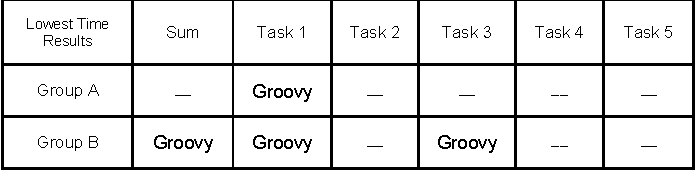
\psfig{file=Development_Time_Results.pdf,width =3.4in}
\caption{Group A(Groovy first) and Group B(Java first); dyn: dynamic type system \cite{Stuchlik2011}}
\label{Relationresults}
\end{figure}

For both groups, no significant positive impact was found for the static type system for any task. Additionally, the amount of time saved ranged from 8 minutes to 37 minutes,for all tasks, though the median of the summed development times for the statically typed task was less than 100 minutes. This can not be explained just by the time taken to write the type casts, and suggests that type systems have some kind of complexity beyond this.

It should be noted that these results only concern trivial programming tasks, and would not apply to non-trivial task. The authors argue that ``as soon as we speak about non-trivial programming tasks, no positive impact [of dynamic types] can be measured.'' Though they do not point to a study that could actually answer this statement, the authors do suggest that further studies need to be conducted in order to verify their hypothesis.
\section{Acknowledgments}

\section{Conclusions}\label{results}


\bibliographystyle{abbrv}
\bibliography{My_paper.bib}


\end{document}
